\documentclass[a4paper,12pt]{article}

%%%%%%%%%%%%%%%%%%%%
%%%%  PREAMBLE  %%%%
%%%%%%%%%%%%%%%%%%%%

\usepackage[T1]{fontenc}
\usepackage[utf8]{inputenc}

\usepackage[english,italian]{babel}

\usepackage{hyperref}
\hypersetup{hidelinks}

\usepackage[margin=2.5cm]{geometry}
\usepackage{minipage-marginpar}
\usepackage{fancyhdr}
\usepackage[bottom]{footmisc}
\usepackage{lastpage}

\usepackage{enumitem}
\usepackage{tabularx}

\usepackage{graphicx}

\setlength{\parindent}{0em}
\setlength{\parskip}{1em}

\fancyhead[L]{\leftmark}
\fancyhead[R]{\shortstack[r]{Versione documento: 0.01 \\ Gruppo: T27}}

\fancyfoot[C]{}
\fancyfoot[R]{\thepage/\pageref{LastPage}}

\renewcommand{\headrulewidth}{2pt}
\renewcommand{\headruleskip}{3pt}
\setlength{\headheight}{30pt}

\renewcommand{\footrulewidth}{2pt}

\setlist[itemize]{itemsep=0.25em,topsep=0pt}
\setlist[enumerate]{itemsep=0.25em,topsep=0pt,align=left}

%%%%%%%%%%%%%%%%%%%%
%%%%  DOCUMENT  %%%%
%%%%%%%%%%%%%%%%%%%%

\title{Web Music Player}
\author{Gruppo T27}

\begin{document}

\pagestyle{empty}

\begin{center}

    \vspace{2 cm}

    \begin{tabular*}{\textwidth}{ c @{\extracolsep{\fill}} c }
        
\includegraphics[width=0.3\textwidth]{marchio_unitrento.pdf} & \shortstack{\Large{Dipartimento di Ingegneria} \\ \Large{e Scienza dell'Informazione}}
    \end{tabular*}

    \vspace{2 cm} 
  
    \LARGE{Ingegneria del software\\}
  
    \vspace{1.5 cm} 
    \Large\textsc{Documento dei requisiti\\} 
    \Large\textsc{Versione: 0.01\\} 
    \vspace{2 cm} 
    \Huge\textsc{Web Music Player\\}
    \Large{\it{Gruppo T27}}
  
    \vspace{2 cm} 
  
    \Large{Anno accademico 2022/2023}
\end{center}

\newpage
\tableofcontents

\pagestyle{fancy}

\newpage
\section{Scopo del documento}

Il presente documento riporta l’analisi dei requisiti di sistema del progetto Web Music Player. Lo scopo di questo di questo documento è quello di:
\begin{itemize}
    \item descrivere gli obiettivi funzionali;
    \item elencare i requisiti non funzionali;
    \item mostrare le interazioni del progetti con altri sistemi;
    \item mostrare le componenti interne del sistema.
\end{itemize}

\newpage
\section{Requisiti funzionali}

Andiamo a descrivere nel dettaglio i requisiti funzionali del sistema. Per fare ciò, sfruttiamo gli use-case diagram, un utile strumento di visualizzazione. Ciascuno use-case diagram sarà accompagnato da una descrizione; questa può essere testuale o tramite un ulteriore diagramma.

\subsection*{RF1 Registrazione}

\begin{figure}[htp]
    \centering
    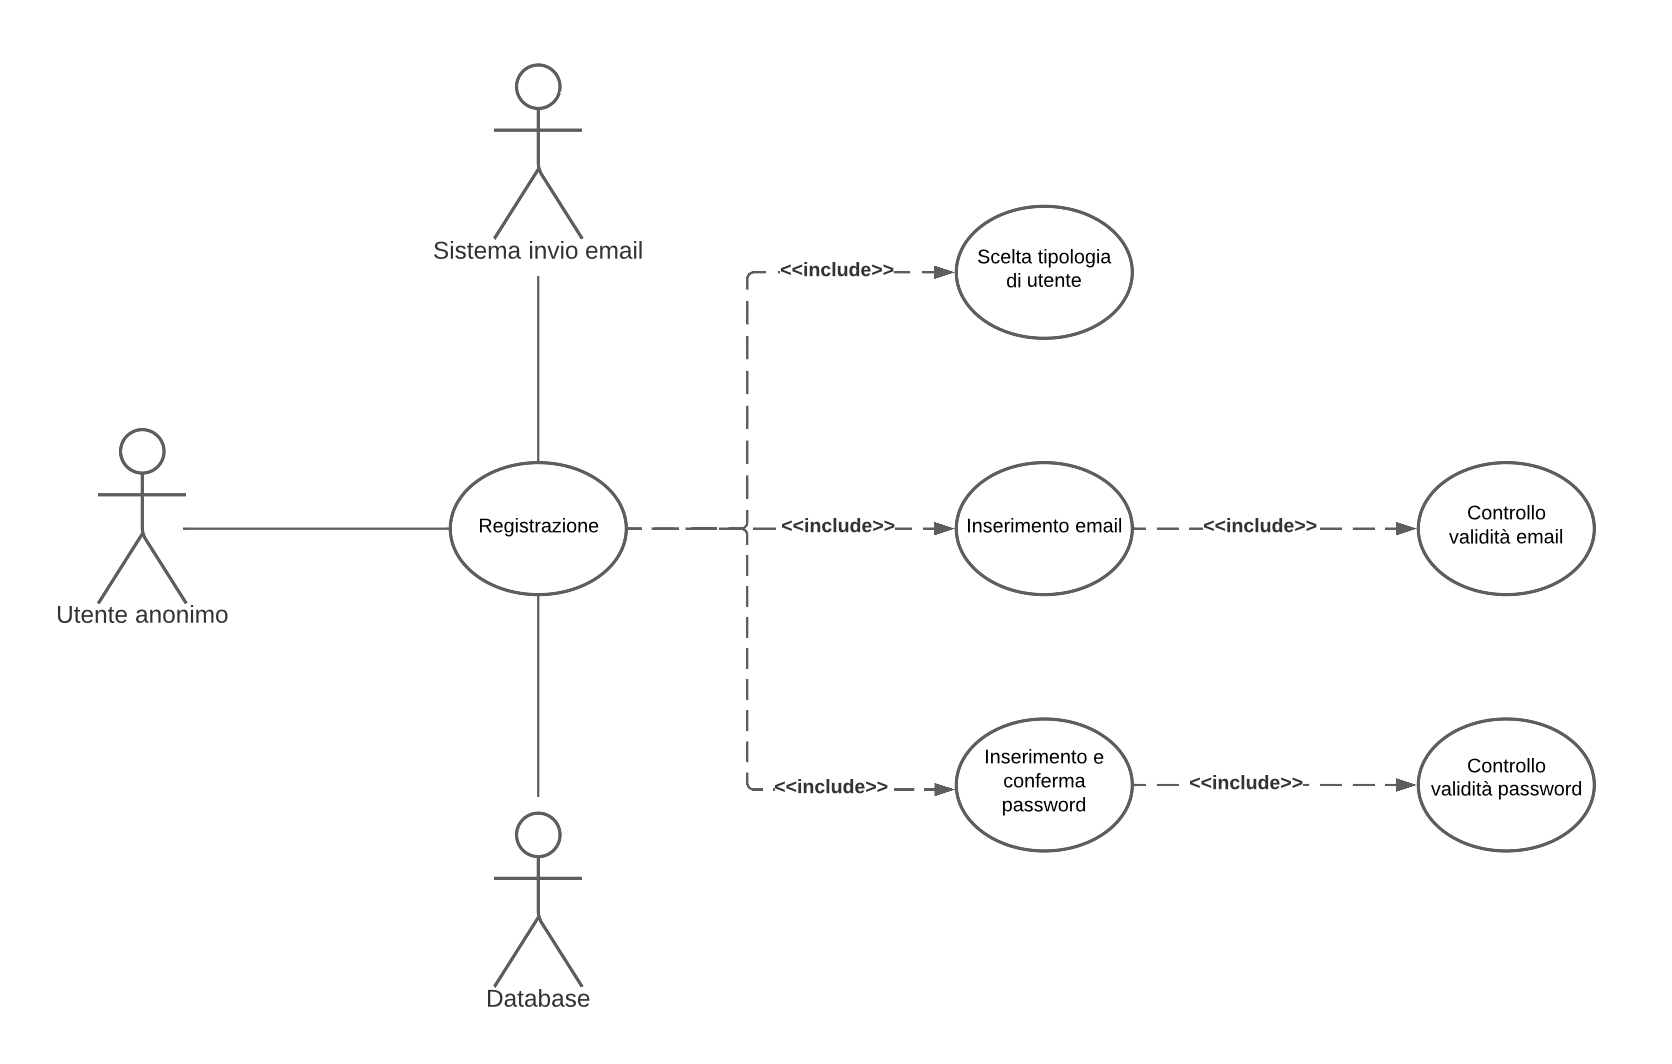
\includegraphics[width=0.75\textwidth]{diagrams/use-case-1.png}
\end{figure}

Per descrivere questo use-case, facciamo uso di un diagramma delle attività:

\begin{figure}[htp]
    \centering
    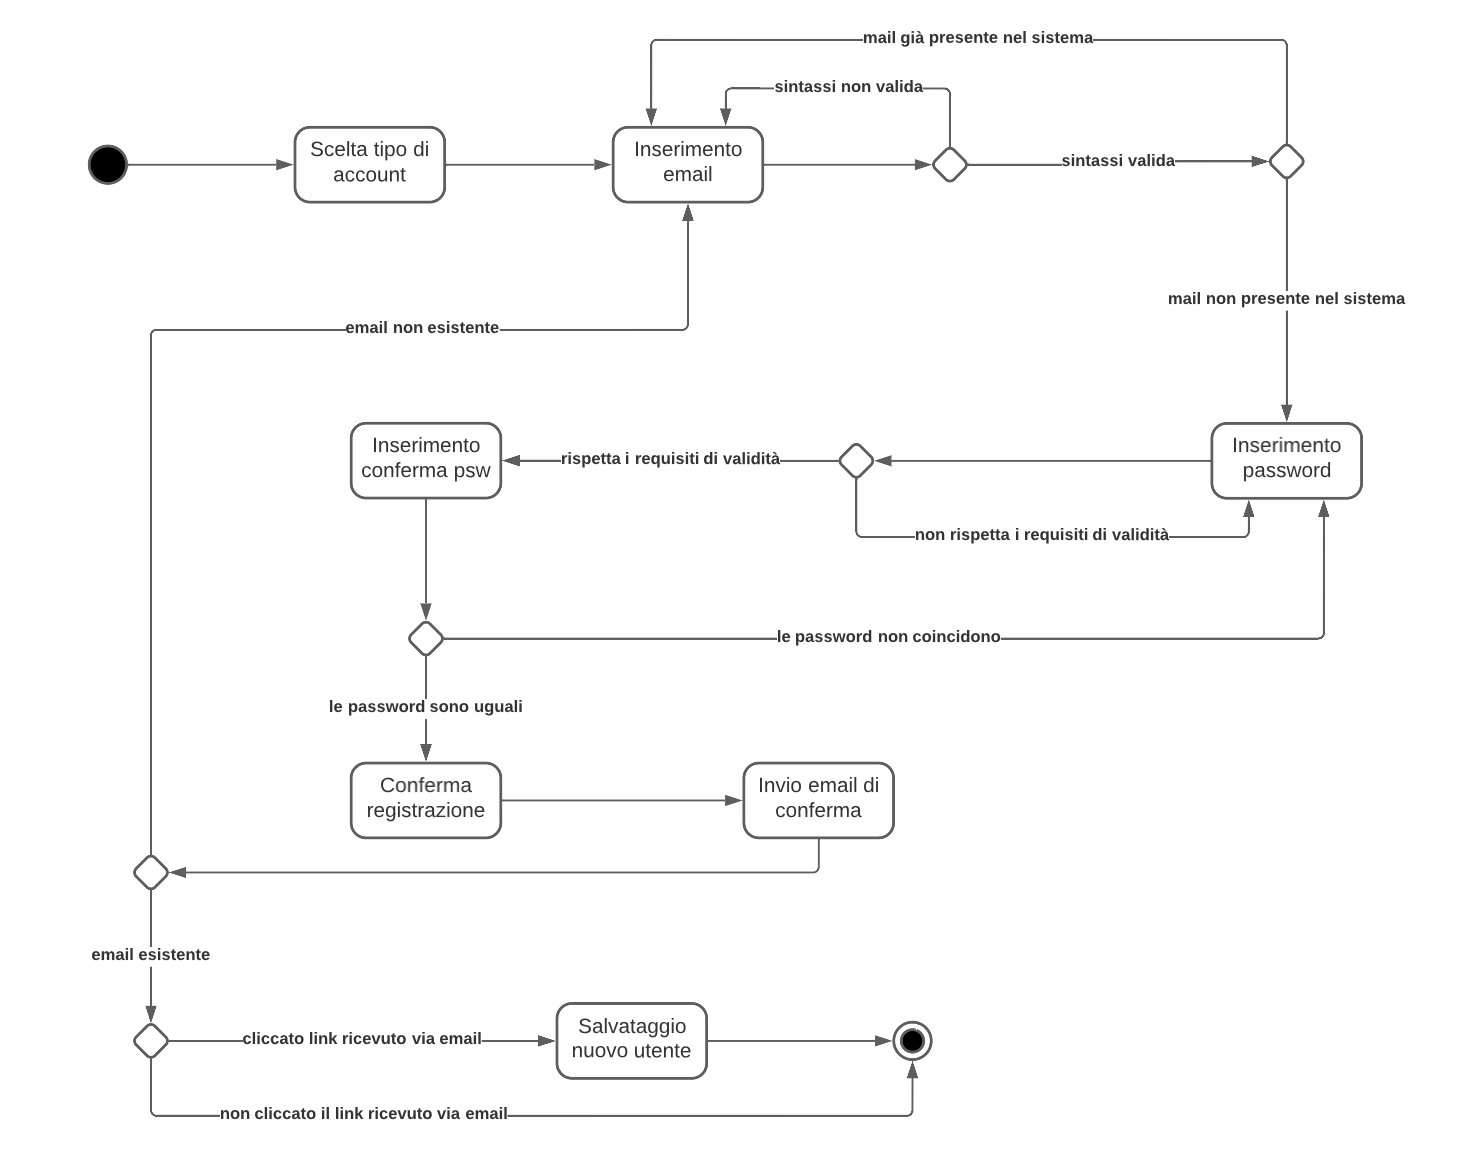
\includegraphics[width=0.75\textwidth]{diagrams/activity-1.png}
\end{figure}

\newpage

\subsection*{RF2 Pagamento}

\begin{figure}[htp]
    \centering
    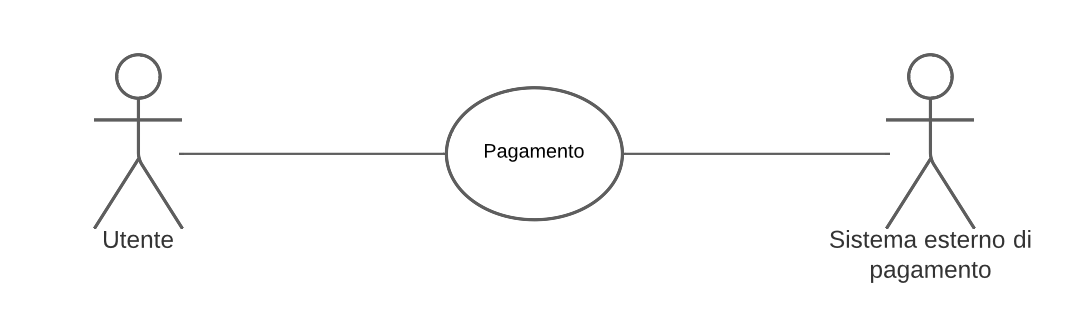
\includegraphics[width=0.75\textwidth]{diagrams/use-case-2.png}
\end{figure}

\textbf{Descrizione:} l'utente paga il servizio tramite un sistema esterno. 

\vspace{1em}
\subsection*{RF3 Login}

\begin{figure}[htp]
    \centering
    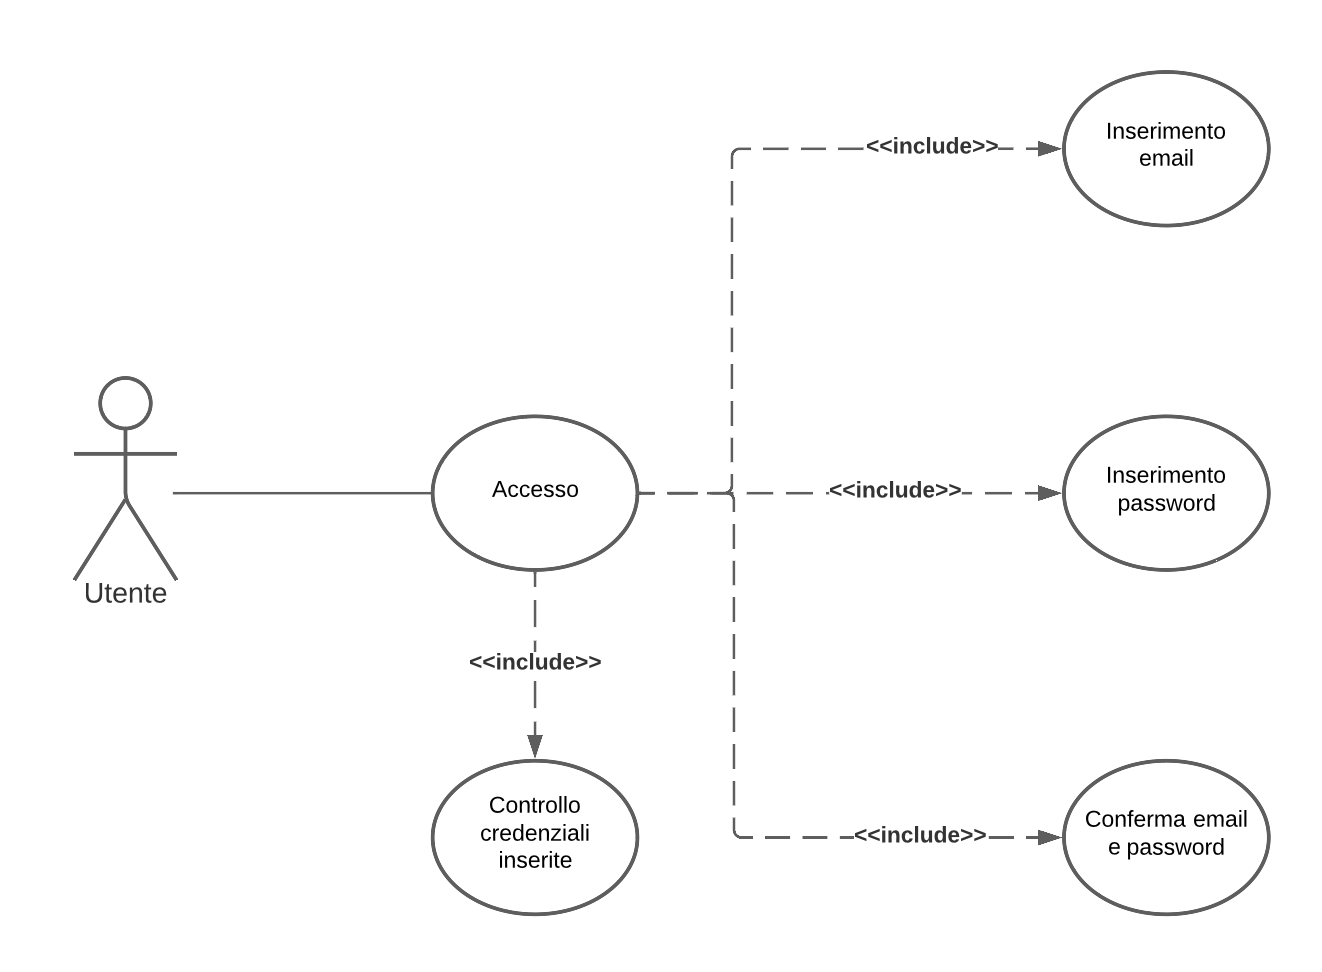
\includegraphics[width=0.75\textwidth]{diagrams/use-case-3.png}
\end{figure}

\textbf{Descrizione:} questo use-case descrivere l’accesso al sito per un utente già registrato.

\textbf{Passi:}
\begin{enumerate}
    \item L’utente inserisce la sua mail 
    \item L’utente inserisce la password associata al suo account 
    \item L’utente conferma la mail e la password inserite
    \item Il sistema verifica la correttezza di mail e password \textbf{[exception 1]}
    \item L’utente entra nel sito
\end{enumerate}

\textbf{[exception 1]} Nel caso in cui l’email e/o la password siano errati viene esposto un messaggio di errore: “email e/o password errati”.

\newpage

\subsection*{RF4 Recupero password}

\begin{figure}[htp]
    \centering
    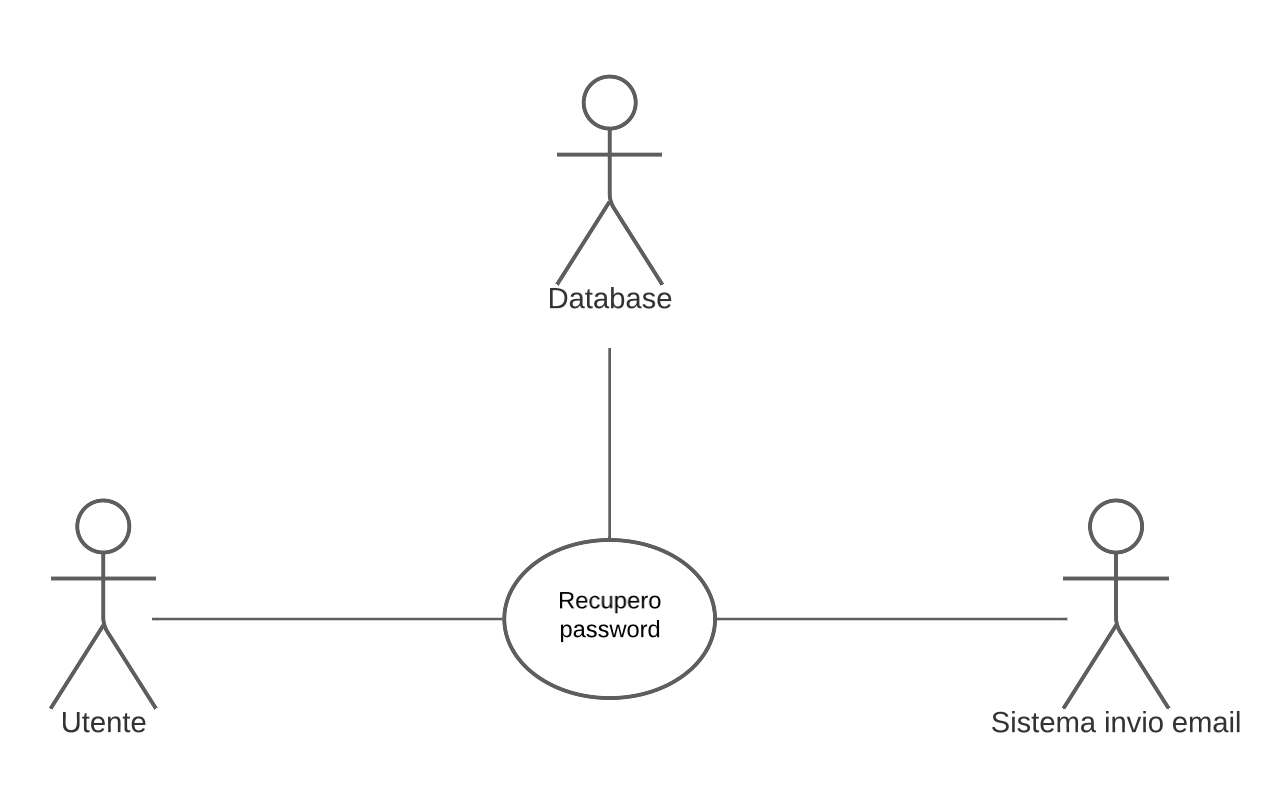
\includegraphics[width=0.75\textwidth]{diagrams/use-case-4.png}
\end{figure}

Per descrivere questo use-case, facciamo uso di un diagramma delle attività:

\begin{figure}[htp]
    \centering
    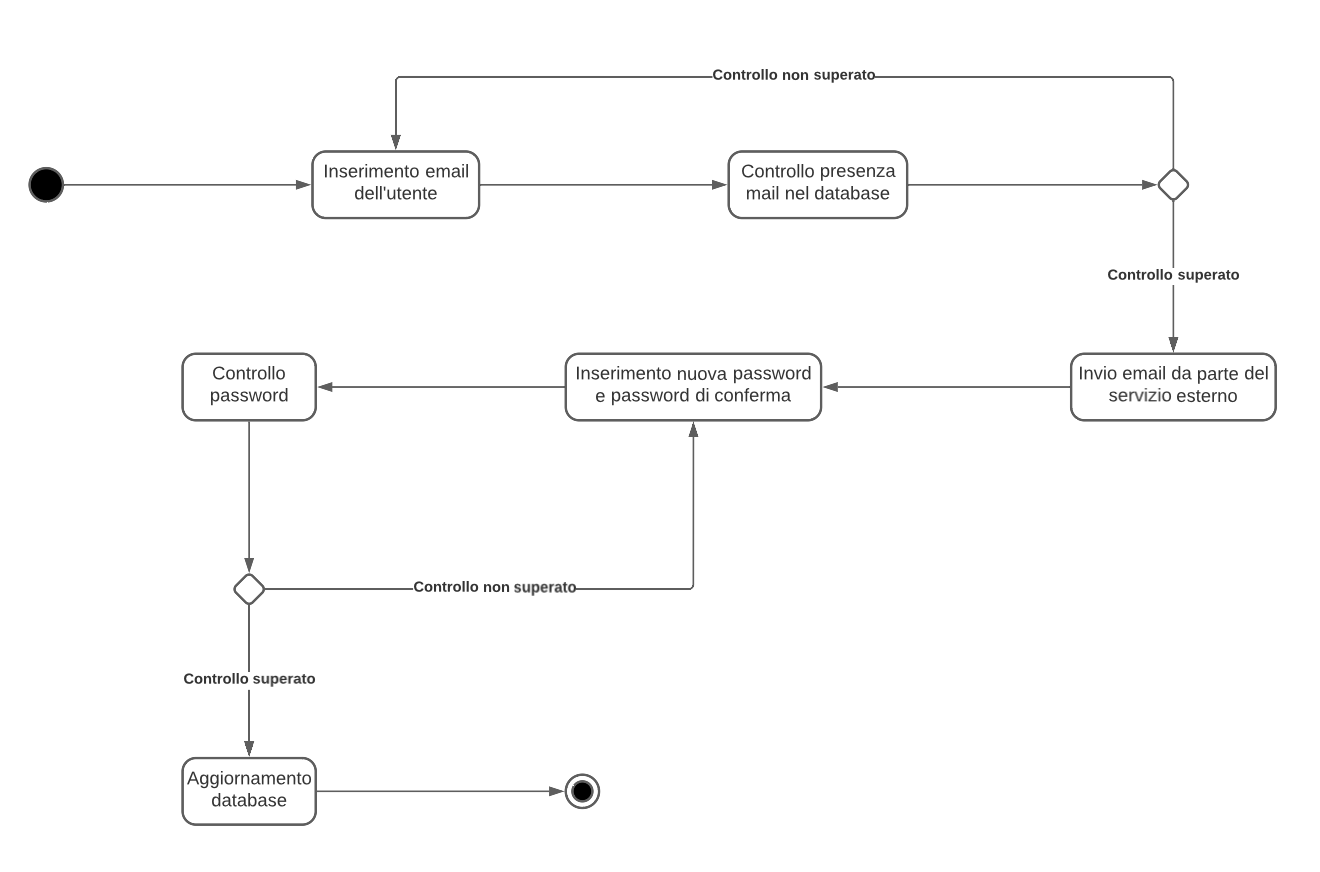
\includegraphics[width=0.75\textwidth]{diagrams/activity-4.png}
\end{figure}

\subsection*{RF 5-13}

\begin{figure}[htp]
    \centering
    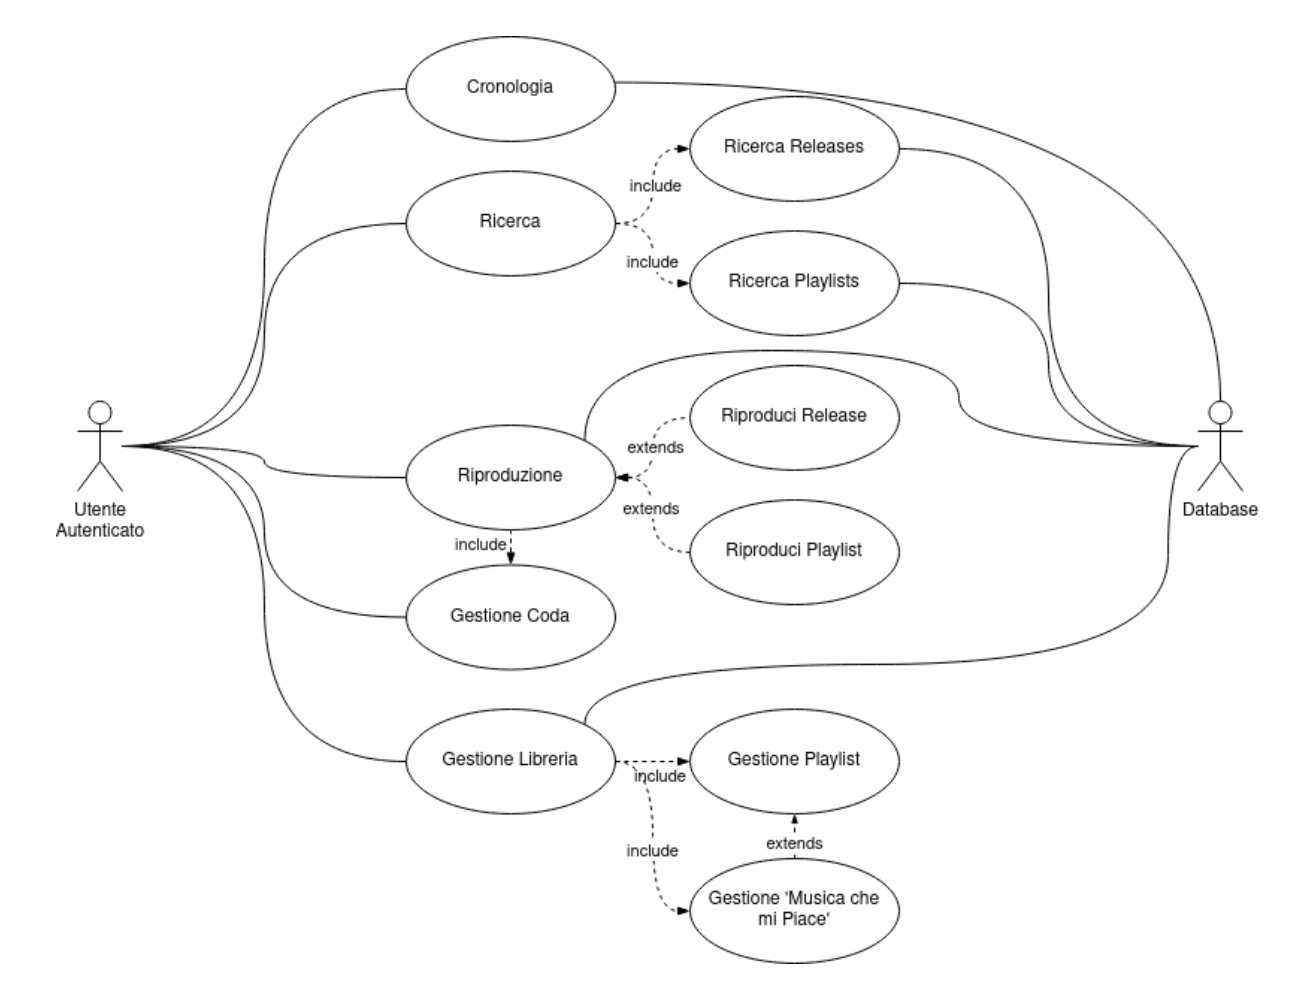
\includegraphics[width=0.75\textwidth]{diagrams/use-case-5-6-7-8-9-10-11-12-13.png}
\end{figure}

\subsubsection*{RF5 Ricerca}
\textbf{Descrizione:} l’utente deve poter ricercare tra releases e le proprie playlists. \newline
\textbf{Passi:}
\begin{enumerate}
    \item L’utente inserisce del testo nella barra di ricerca
    \item Il sistema ricerca in modo approssimato tra le releases caricate e le playlist e restituisce una lista di risultati, ordinati in base a quello più vicino alla query
\end{enumerate}

\subsubsection*{RF 6 Riproduzione}

\textbf{Descrizione:} l’utente deve poter riprodurre una release o una playlist a partire da un brano e avere quelli successivi automaticamente messi nella coda di riproduzione nel corretto ordine. \newline
\textbf{Passi:}
\begin{enumerate}
    \item L’utente preme sull’apposito pulsante per iniziare la riproduzione del brano \textbf{[extension 1]}
    \item Il client dialoga col sistema per iniziare lo stream
    \item Il sistema inoltre aggiunge la playlist o release alla cronologia
\end{enumerate}
\textbf{[extension 1]} Se il brano si trova in una playlist e non è l’ultimo, il client si dovrà premurare di aggiungere anche i brani che vengono dopo alla coda nello stesso ordine in cui appaiono nella playlist. Similmente, se il brano viene riprodotto come parte di una release e non è l’ultimo, il client dovrà aggiungere alla coda i brani che succedono quello riprodotto nell’ordine corretto.

\subsubsection*{RF 7 Coda}

\textbf{Descrizione:} l’utente deve poter gestire la propria coda di riproduzione (riordinarla, rimuovervi brani e aggiungerne) e il client deve seguire la coda per sapere l’ordine in cui vanno riprodotte le canzoni. \newline
\textbf{Passi:}
\begin{enumerate}
    \item L’utente, attraverso appositi pulsanti, è in grado di riordinare, rimuovere e aggiungere brani alla coda
    \item Il client, unico posto dove la coda è mantenuta, deve salvare ogni modifica
    \item Una volta che la riproduzione del brano corrente è terminata, la coda va utilizzata per trovare il prossimo brano da riprodurre
\end{enumerate}

\subsubsection*{RF 8 Libreria}

\textbf{Descrizione:} l’utente deve poter vedere le proprie playlists e la musica che ha salvato.

\subsubsection*{RF 9 Musica che ti piace}

\textbf{Descrizione:} l’utente deve poter salvare le releases che ascolta in una raccolta speciale chiamata “Musica che ti Piace” e successivamente deve essere in grado di gestire (rimuovere, riordinare o aggiungere releases) suddetta raccolta. \newline
\textbf{Passi:}
\begin{enumerate}
    \item Durante la riproduzione di un brano o altri momenti, l’utente potrà, attraverso un apposito pulsante, chiedere al sistema di aggiungere una release alla raccolta “Musica che ti piace” dell’utente
    \item Successivamente, da apposite tab, è possibile, utilizzando appositi pulsanti, dialogare col sistema per riordinare o rimuovere releases dalla raccolta
\end{enumerate}

\subsubsection*{RF 10 Playlist}

\textbf{Descrizione:} l’utente deve poter salvare i brani che ascolta in raccolte chiamate playlists e successivamente deve essere in grado di gestirle (rimuovere, riordinare o aggiungere releases e rimuovere playlists). \newline
\textbf{Passi:}
\begin{enumerate}
   \item Durante la riproduzione di un brano o altri momenti, l’utente potrà, attraverso un apposito pulsante, chiedere al sistema di aggiungere un brano a una delle playlists che ha già creato o in una nuova, a cui deve dare un nome
    \item Successivamente, da apposite tab, è possibile, utilizzando appositi pulsanti, dialogare col sistema per riordinare o rimuovere le releases di una playlist o per rimuovere interamente una playlist
\end{enumerate}

\subsubsection*{RF 11 Consigliati}

\textbf{Descrizione:} Il sistema suggerirà all’utente releases dal proprio database, con l'obiettivo di consigliargli brani che possano piacergli.

\subsubsection*{RF 12 Feedback}

\textbf{Descrizione:} l’utente deve essere in grado di poter restituire al sistema feedback riguardo i consigli, per aiutarlo nel perfezionamento di futuri consigli. \newline
\textbf{Passi:}
\begin{enumerate}
   \item L’utente si vedrà arrivare dei consigli dal sistema, grazie agli appositi pulsanti sarà in grado di riprodurre la release consigliata e segnalare al sistema se questa era di suo gradimento o meno
\end{enumerate}

\subsubsection*{RF 13 Cronologia}

\textbf{Descrizione:} l’utente deve poter recuperare la lista delle ultime 30 riproduzioni (siano esse releases o playlist). \newline
\textbf{Passi:}
\begin{enumerate}
    \item L’utente si reca sul menù dedicato alla cronologia
    \item Il sistema recupera la lista delle ultime 30 riproduzioni e le mostra all’utente
\end{enumerate}

\subsection*{RF 14-17}

\begin{figure}[htp]
    \centering
    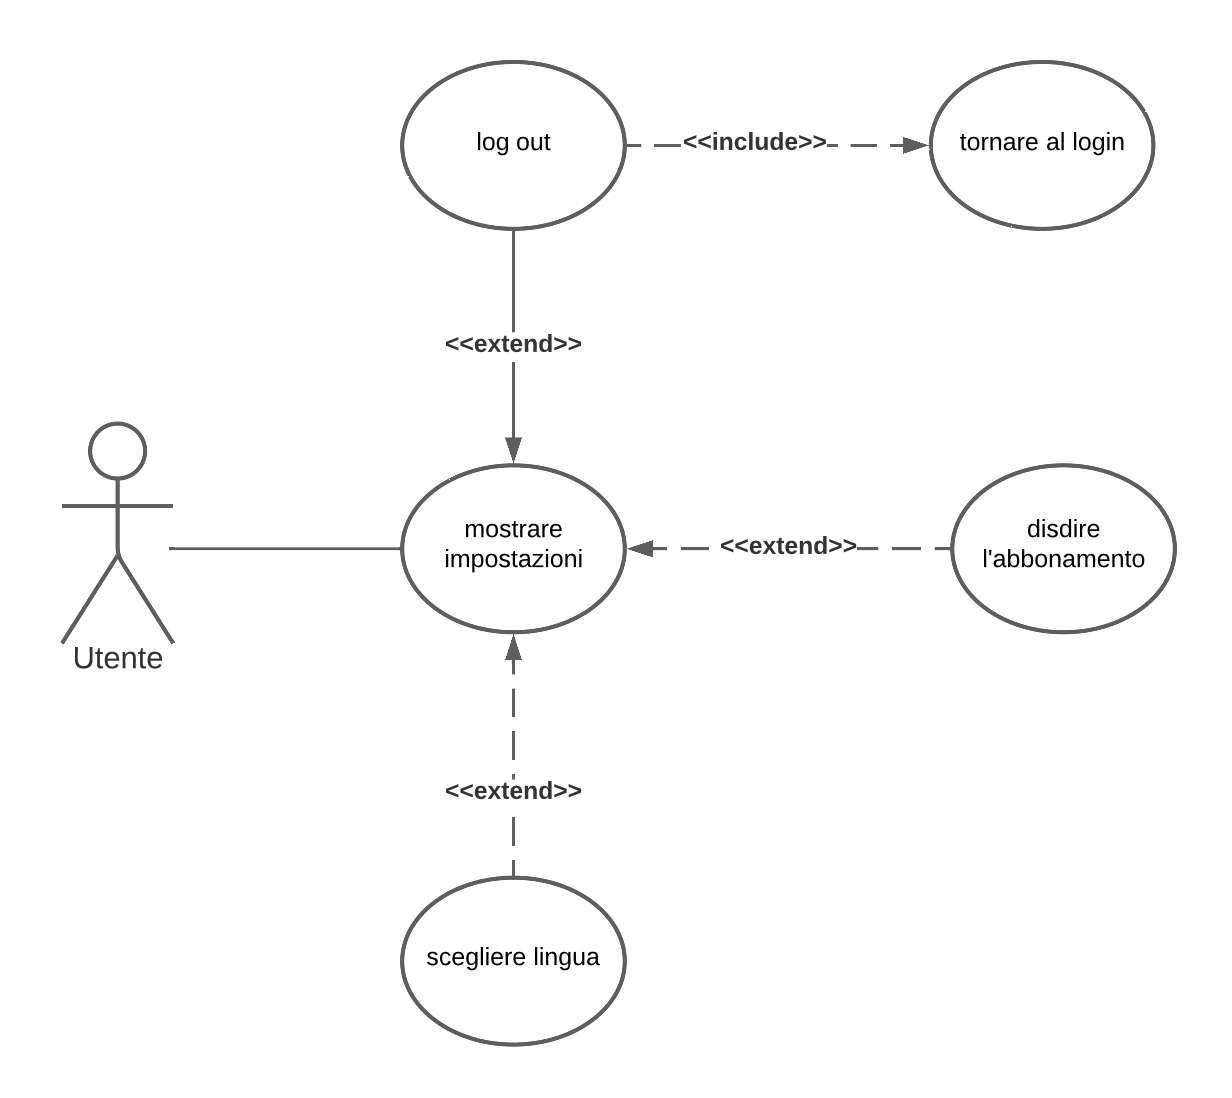
\includegraphics[width=0.75\textwidth]{diagrams/use-case-14-15-16-17.png}
\end{figure}

\subsubsection*{RF 14 Impostazioni}

\textbf{Descrizione:} l’utente può accedere alla pagina delle impostazioni, dalla quale può compiere una serie di azioni relative al proprio account e alla piattaforma.

\subsubsection*{RF 15 Logout}

\textbf{Descrizione:} l’utente può disconnettersi dalla piattaforma. \newline
\textbf{Passi:}
\begin{enumerate}
    \item L’utente si reca alla pagina delle impostazioni
    \item L’utente preme un pulsante per effettuare la disconnessione del proprio account
    \item L’utente viene riportato alla pagina di login
\end{enumerate}

\subsubsection*{RF 16 Disdire l'abbonamento}

\textbf{Descrizione:} l’utente può disconnettersi dalla piattaforma. \newline
\textbf{Passi:}
\begin{enumerate}
    \item L’utente si reca alla pagina delle impostazioni
    \item L’utente preme un pulsante per terminare l’abbonamento alla piattaforma
    \item L’utente potrà usufruire del servizio fino al termine del mese per il quale ha pagato
    \item Una volta terminato quel periodo, dopo l’accesso alla piattaforma l’utente sarà portato alla pagina del pagamento
\end{enumerate}

\subsubsection*{RF 17 Cambio lingua}

\textbf{Descrizione:}  l’utente può cambiare la lingua della piattaforma. \newline
\textbf{Passi:}
\begin{enumerate}
    \item L'utente si reca alla pagina delle impostazioni
    \item L’utente tramite un menù a tendina può scegliere la lingua di visualizzazione della piattaforma
    \item Il servizio si adatta, modificando i vari campi testuali per riflettere la lingua selezionata dall’utente
\end{enumerate}

\subsection*{RF 18-19}

\begin{figure}[htp]
    \centering
    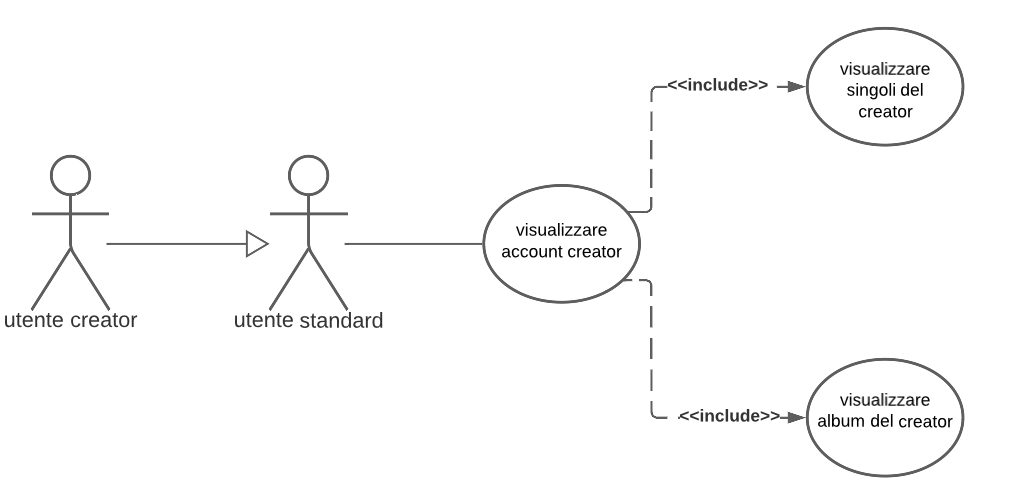
\includegraphics[width=0.75\textwidth]{diagrams/use-case-18-19.png}
\end{figure}

\subsubsection*{RF 18 Account creator}

\textbf{Descrizione:} l’account creator consiste in un'estensione dell'account standard.

\subsubsection*{RF 19 Visualizzare account creator}

\textbf{Descrizione:} gli utenti creator e gli utenti standard possono visualizzare le pagine degli account creator. Qui sono presenti due elenchi: i singoli caricati e gli album caricati da quel creator.

\subsection*{RF20 Caricare releases}

\begin{figure}[htp]
    \centering
    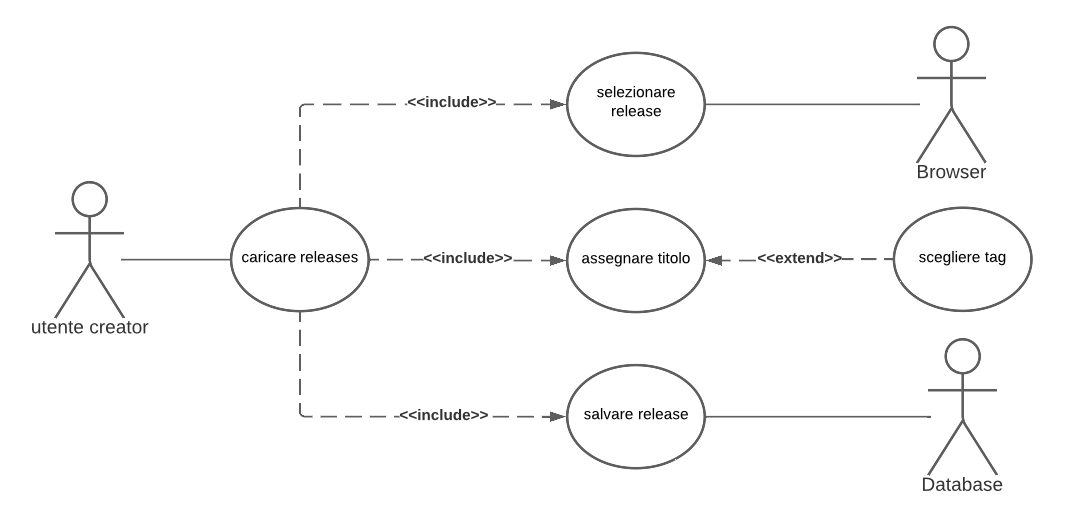
\includegraphics[width=0.75\textwidth]{diagrams/use-case-20.png}
\end{figure}

\textbf{Descrizione:} questo use case descrive il caricamento delle releases sulla piattaforma da parte dei creator.

\textbf{Passi:}
\begin{enumerate}
    \item L’utente creator sceglie di caricare una release dalla sua pagina
    \item L’utente creator seleziona la release da caricare tramite il browser
    \item L’utente creator sceglie il titolo da assegnare alla release \textbf{[extension 1]}
    \item L’utente creator conferma la scelta
    \item La release viene salvata sul database della piattaforma
\end{enumerate}
\textbf{[extension 1]} L’utente creator può aggiungere dei tag alla release caricata.

\subsection*{RF21 Modificare releases}

\begin{figure}[htp]
    \centering
    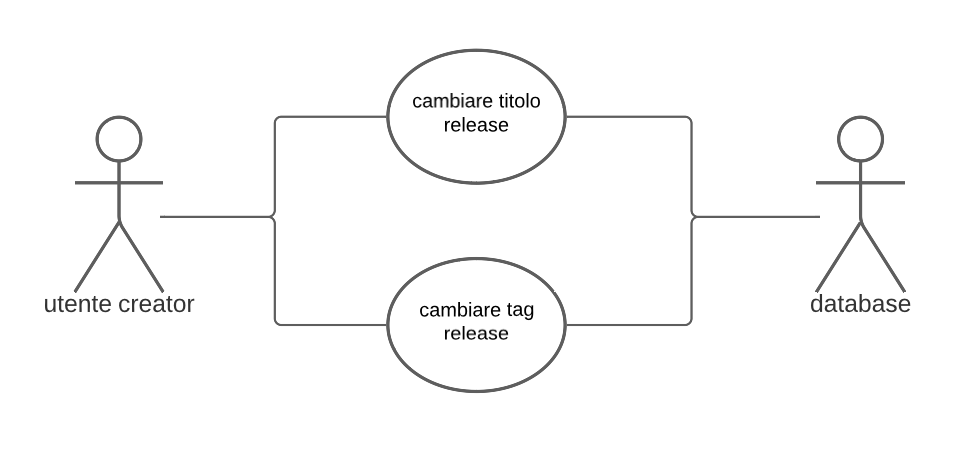
\includegraphics[width=0.75\textwidth]{diagrams/use-case-21.png}
\end{figure}

\textbf{Descrizione:} gli utenti creator possono modificare il titolo e i tag delle releases che hanno caricato sulla piattaforma. Questo dalla schermata del loro account.

\textbf{Passi:}
\begin{enumerate}
    \item L’utente creator seleziona una release dalla propria pagina
    \item L'utente sceglie l’opzione di modifica
    \item L'utente può da qui modificare il titolo, i tag, o entrambi
    \item Le modifiche vengono salvate nel database
    
\end{enumerate}

\subsection*{RF22 Eliminare releases}

\begin{figure}[htp]
    \centering
    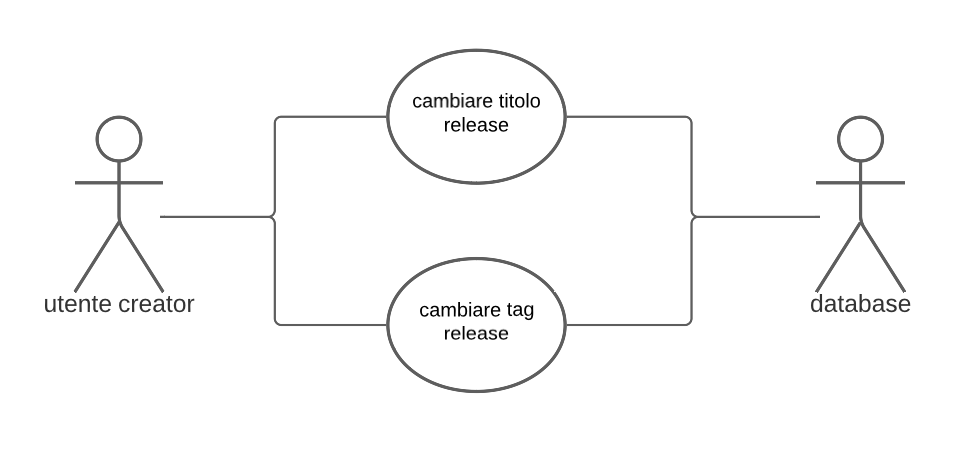
\includegraphics[width=0.75\textwidth]{diagrams/use-case-22.png}
\end{figure}

\textbf{Descrizione:} gli utenti creator possono cancellare dalla piattaforma releases da loro caricate. Questo dalla schermata del loro account.

\textbf{Passi:}
\begin{enumerate}
    \item L’utente creator seleziona una release dalla propria pagina
    \item L'utente sceglie l’opzione di eliminazione
    \item L'utente conferma l’eliminazione della release dalla piattaforma
    \item La release viene rimossa dal database    
\end{enumerate}

\newpage
\section{Requisiti non funzionali}

Presentiamo i requisiti non funzionali del progetto. Ciascun requisito è accompagnato da una misura che, quando raggiunta, trasmette se il corrispondente requisito è stato raggiunto.

\subsection*{Portabilità}

{
    \centering
    \begin{tabularx}{\textwidth}{|l|>{\raggedright\arraybackslash}X|>{\raggedright\arraybackslash}X|>{\raggedright\arraybackslash}X|}
    \hline
    Portabilità & Il servizio deve essere accessibile dai browser di computer fissi e portatili. Deve supportare i principali browser in commercio. & Le versioni dei browser Safari, Edge, Firefox, Chrome, rilasciate entro il 2017 devono supportare le funzionalità del software. \\
    \hline
    \end{tabularx} \par
}
\subsection*{Security}
{
    \centering
    \begin{tabularx}{\textwidth}{|l|>{\raggedright\arraybackslash}X|>{\raggedright\arraybackslash}X|>{\raggedright\arraybackslash}X|}
    \hline
    Password sicura & Gli utenti possono associare al proprio account solamente una password sicura. & Per essere classificata come sicura, la password deve avere una lunghezza minima di 8 caratteri, una lettera maiuscola, una lettera minuscola, un carattere speciale (\%\&\#!@*\textasciicircum). \\
    \hline
    Email verificata & L’indirizzo email inserito dall’utente deve essere verificato come esistente e in suo possesso. & Quando l’utente clicca il pulsante per la registrazione, una mail viene inviata all’indirizzo inserito dall’utente contenente un link da cliccare. Una volta cliccato il link, la mail viene validata. \\
    \hline
    Protezione della trasmissione & La trasmissione dati tra il browser dell’utente e il server web del sistema deve essere cifrata. & Deve essere usato il protocollo https. \\
    \hline
    Protezione diritti d'autore & Il software deve fare il possibile per prevenire la diffusione non autorizzata delle releases disponibili. & \\
    \hline
    \end{tabularx} \par
}
\subsection*{Recupero password}

{
    \centering
    \begin{tabularx}{\textwidth}{|l|>{\raggedright\arraybackslash}X|>{\raggedright\arraybackslash}X|>{\raggedright\arraybackslash}X|}
    \hline
    Recupero password & L’utente deve essere in grado di accedere al suo account anche nel caso in cui abbia dimenticato la password. & Nella pagina di registrazione è disponibile un bottone per recuperare la password attraverso l’indirizzo email associato all’account. \\
    \hline
    \end{tabularx} \par
}
\subsection*{Cambiare la password}

{
    \centering
    \begin{tabularx}{\textwidth}{|l|>{\raggedright\arraybackslash}X|>{\raggedright\arraybackslash}X|>{\raggedright\arraybackslash}X|}
    \hline
    Cambiare la password & L’utente loggato deve essere in grado di cambiare la password associata al suo account. & Dalle impostazioni dev’essere possibile inserire una nuova password per sostituire quella corrente. \\
    \hline
    \end{tabularx} \par
}
\subsection*{Affidabilità}

{
    \centering
    \begin{tabularx}{\textwidth}{|l|>{\raggedright\arraybackslash}X|>{\raggedright\arraybackslash}X|>{\raggedright\arraybackslash}X|}
    \hline
    Ridondanza & L’infrastruttura è ridondata per garantire la protezione dal fallimento dei dischi. & Devono essere presenti almeno due istanze del servizio, per cui la terminazione di una non intacchi la disponibilità del servizio. La perdita di servizio dev’essere automaticamente segnalata all’amministratore. \\ \hline
    Backup & Devono essere presenti dei backup del sito in modo da recuperare i dati in caso di guasti o attacchi hacker. & I backup devono comprendere tutti i dati del sistema. Sono eseguiti mensilmente. Sono salvati su un servizio esterno. \\
    \hline
    \end{tabularx} \par
}
\subsection*{Usabilità}

{
    \centering
    \begin{tabularx}{\textwidth}{|l|>{\raggedright\arraybackslash}X|>{\raggedright\arraybackslash}X|>{\raggedright\arraybackslash}X|}
    \hline
    Familiarità & L’applicazione deve risultare familiare e facile da utilizzare. & Giovani adulti di età compresa tra i 16 e i 35 anni, previa esperienza di un recente dispositivo digitale (dal 2015 in poi) devono riuscire ad usufruire del servizio senza necessitare di aiuto esterno (almeno 50 utenti di test). \\
    \hline
    \end{tabularx} \par
}
\subsection*{Privacy}

{
    \centering
    \begin{tabularx}{\textwidth}{|l|>{\raggedright\arraybackslash}X|>{\raggedright\arraybackslash}X|>{\raggedright\arraybackslash}X|}
    \hline
    GDPR & Conforme al regolamento generale sulla protezione dei dati in sigla GDPR, ufficialmente regolamento n. 2016/679. & Il software permette la cancellazione dei dati personali che lo riguardano senza ingiustificato ritardo. Permette inoltre all’utente di ottenere la conferma che sia o meno in corso un trattamento di dati personali che lo riguardano. \\
    \hline
    \end{tabularx} \par
}
\subsection*{Performance}

{
    \centering
    \begin{tabularx}{\textwidth}{|l|>{\raggedright\arraybackslash}X|>{\raggedright\arraybackslash}X|>{\raggedright\arraybackslash}X|}
    \hline
    Qualità dell'audio & Lo streaming deve adattarsi alla banda disponibile all’utente. & Il servizio deve garantire lo streaming ad un minimo 160 kbps di banda e fino ad un massimo di 320 kbps. \\ \hline
    Velocità di ricerca & La ricerca all’interno del sistema deve avvenire in un tempo accettabile. & I risultati dalla barra di ricerca vengono restituiti entro 10 secondi, con una media di 3 secondi. \\
    \hline
    \end{tabularx} \par
}
\subsection*{Pagamento}

{
    \centering
    \begin{tabularx}{\textwidth}{|l|>{\raggedright\arraybackslash}X|>{\raggedright\arraybackslash}X|>{\raggedright\arraybackslash}X|}
    \hline
    Pagamento & Si usufruisce al servizio sulla base di un pagamento ricorrente. & Il pagamento avviene mensilmente; il giorno corrisponde al giorno della sottoscrizione al servizio da parte dell’utente. La piattaforma sfrutta il servizio di pagamento scelto dall’utente per prelevare la quota necessaria. \\
    \hline
    \end{tabularx} \par
}
\subsection*{Tag}

{
    \centering
    \begin{tabularx}{\textwidth}{|l|>{\raggedright\arraybackslash}X|>{\raggedright\arraybackslash}X|>{\raggedright\arraybackslash}X|}
    \hline
    Tag & Ogni release possiede dei tag che la caratterizzano. & Ciascuna release deve essere associata ad un minimo di 3 (tre) tag. \\
    \hline
    \end{tabularx} \par
}

\newpage
\section{Diagramma di contesto}

\newpage
\section{Diagramma delle componenti}

\end{document}